\section{Conclusions}\label{sec:conclusions}
    Now, more than ever, there is a great need for humans to be able to trust the AIAs that we are creating. Assurances are the method by which AIAs can encourage humans to trust them appropriately, and to then use them appropriately. We have presented here a definition, case for, and survey of assurances in the context of human-AIA trust relationships. As a result, important considerations for designing assurances have been laid out and discussed.
    
    The survey was performed, to some extent, from a standpoint of designing an unmanned ground vehicle that is working in concert with a human supervisor. However, the theoretical framework, and classification of assurances is meant to be general in order to apply to a broad range of AIAs.

    There is a fairly large body of research that is focused, in some way, on influencing trust in human-AIA relationships. However, there is a larger portion of research that deals with techniques that would be useful in designing assurances, but that has not directly or consciously considered affecting human-AIA trust through assurances as a formal design goal. Research from these areas (such as V\&V, active learning, and safety) should provide a rich collection of methods to be studied and formally applied to human-AIA trust relationships.

    While the basic definition of assurances (i.e. feedback to user trust, in the human-AIA trust cycle) is simple from a theoretical standpoint, the exercise of gathering related literature helped to illuminate some important considerations and details regarding the design of assurances. The components of Figure \ref{fig:refined_assurances} help to guide the design of assurances for human-AIA trust relationships.

    Generally, we found that designers must consider how the affect of assurances will be measured, how to plan and calculate assurances, what mediums and methods to use, what limitations the AIA has on its ability to express an assurance, and different limitations of human users that need to be considered. Some areas for further research have been noted.

    % \subsection{A Note Regarding Distrust}
    For completeness it is important to mention distrust. As reviewed and discussed by \citet{Lewicki1998-ox}, and formalized in \cite{McKnight2001-hm,McKnight2001-gz} low trust is not the same as distrust, neither is low distrust the same as trust. \citet{McKnight2001-gz} suggest that ``the emotional intensity of distrust distinguishes it from trust''. They explain that distrust comes from emotions like: wariness, caution, and fear. Whereas, trust stems from emotions like: hope, safety, and confidence. Trust and distrust are orthogonal elements that define a person's TRB towards a trustee. %\citet{Lewicki1998-ox} list several behaviors that stem from different combinations of trust and distrust; these are shown in Figure \ref{fig:distrust_table}.
%
    % \begin{figure}[!htbp]
        % \centering
        % 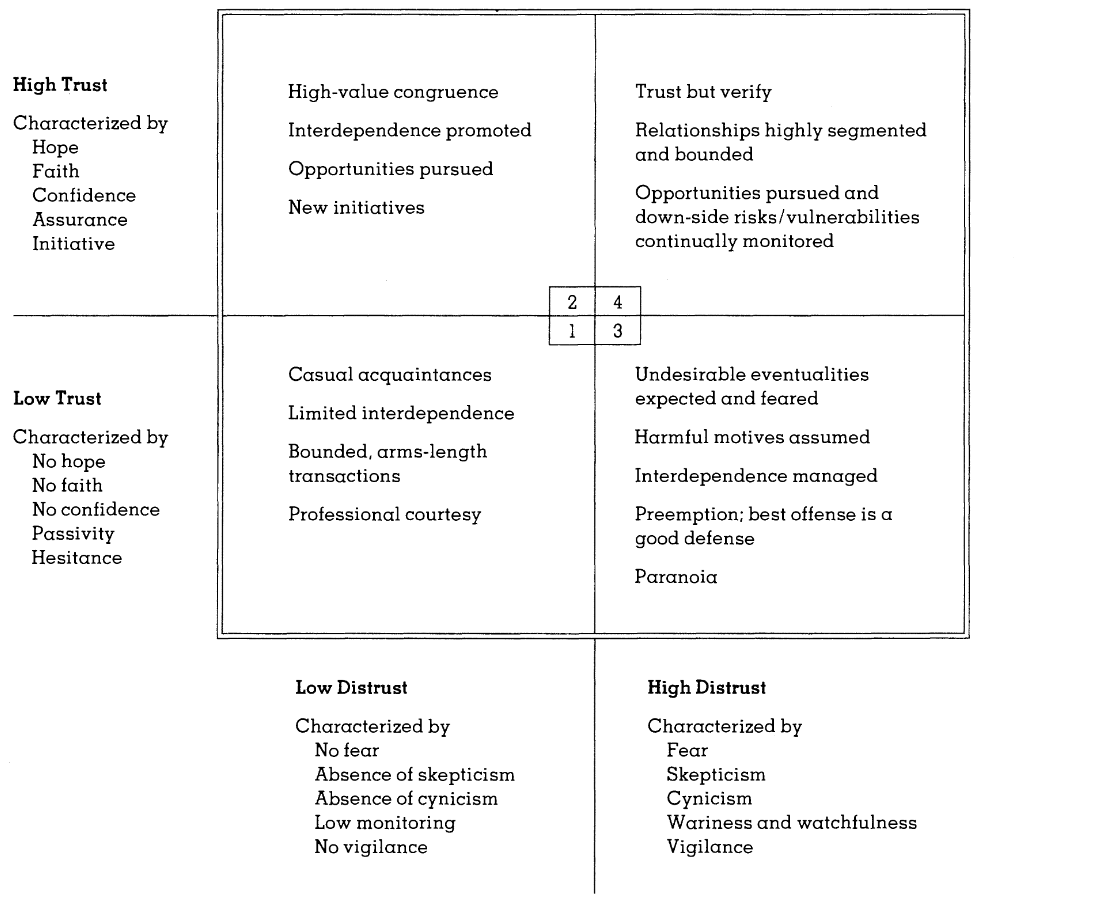
\includegraphics[width=0.6\textwidth]{Figures/distrust_table}
        % \caption{Trust--Distrust table from \cite{Lewicki1998-ox}}
        % \label{fig:distrust_table}
    % \end{figure}

    % In \citet{McKnight2001-gz} models for trust and distrust are proposed, and in later studies empirical evidence to validate some of the dimensions of both models was performed. \citet{McKnight2002-qx} is an empirical study that validates the model and quantifies the relationships between the model dimensions, and \citet{McKnight2004-vv} investigates and quantifies the relationship between dispositional distrust and web-site usage. Finally, \citet{McKnight2006-ce} revisits the position of \citet{McKnight1998-ty} and concludes that research had largely confirmed the model.

    % \textbf{add a small mention of McKnight's definition that distrust is the total opposite of trust?}

    In this survey distrust was not considered; this was in a effort to reduce the scope, which is already at risk of being too large. However, it must be made clear that any \emph{complete} treatment of trust relationships, and for our purposes, designed assurances, must consider the dimensions of distrust as well as those of trust. 
    
    Distrust has been shown to vary with perceived risk \cite{McKnight2004-vv}. This means that the implicit assumption of this paper is that risk in 1-on-1 human-AIA relationships is held constant. We claim that this is a realistic assumption for many practical applications.



\newpage

